\section{Aufbau}
\label{sec:Aufbau}
Der Versuchsaufbau ist in \autoref{fig:Schaltbild} dargestellt. 
\begin{figure}[H]
    \centering
    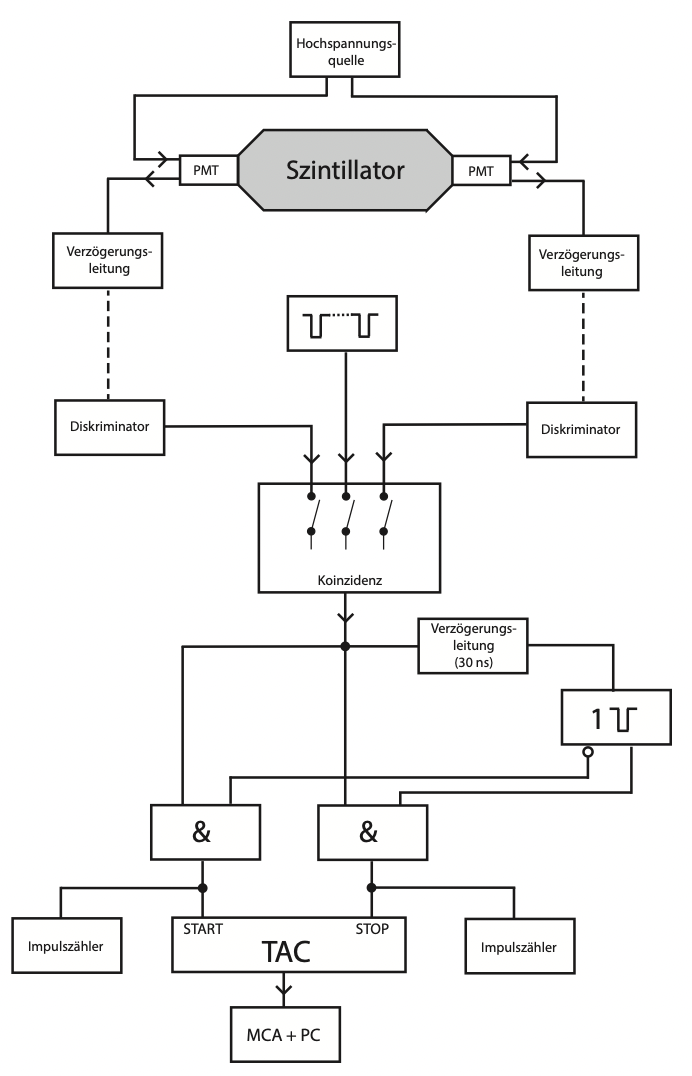
\includegraphics[width=0.5\textwidth]{Abbildungen/Schaltung.png}
    \caption {Schematische Dastellung des Versuchsaufbaus.\cite{V01}}
    \label{fig:Schaltbild}
\end{figure}
Dabei besteht der Versuchsaufbau aus einem Szintillatortank, welcher ein Volumen von ungefähr $\qty{50}{\liter}$.
An beiden Ausgängen des Szintillatortanks ist je ein Photomultiplier (PMT), welcher dazu da ist schwache Lichtsignale durch Erzeugung und Verstärkung eines elektrischen Signals zu detektieren.
Dessen Ausgänge werden über eine Verzögerungsleitung auf den den Eingang eines Diskriminators gegeben, dieser besitzt eine variable Schwelle. 
Anschließend gelangt beide Signale in eine Koinzidenzschaltung, welche nur ein Ausgangssignal erzeugt, wenn beide Signale zeitgleich an ihrem Eingang eintreffen.\\
Danach folgt das ekejtronische Äquivalent zu einer Stoppuhr.
Das Ausgangsignal der Koinzidenz gelangt zu zwei AND-Gattern und über eine weitere Verzögerungsleitung ($\qty{30}{\nano\second}$) zu einem Monoflop. Dieser gibt die Suchzeit $T_S$ vor.
Aufgrund der Verbindung der AND-Gitter mit dem Time-Amplitude-Converter (TAC), startet die Zeitessung aufgrund einem Signal des einem AND-Gitter,
wenn ein Myon das aktive Volumen betritt, und stoppt aufgrund einem Signal des anderem AND-Gitter, wenn das Myon zerfällt. 
Die Start- und Stoppimpulse werden gezählt, indem die Gitter außerdem mit einem Impulsmesser verbunden sind.
Das Signal des TAC gelangt über einem Vielkanalanalysator bzw. Multi-Channel-Analyser (MCA) zu einem PC, wobei es durch eine bestimmte Messsoftware augelesen wird.
Das MCA kann über einen Doppelimpulsgenerator kalibriert werden. Dieser Doppelimpulsgenerator generiert dabei Doppelimpulse mit einem variablen Zeitabstand bei einer Frequenz von $\qty{1}{\kilo\Hz}$.


\section{Durchführung}
\label{sec:Durchführung}
Für die Durchführung des Versuchs muss die Schaltung in \autoref{sec:Aufbau} aufgebaut werden und kalibriert werden.
Dabei wird zur Überprüfung ein Oszilloskop benutzt.\\
Zur Bestimmung der Schwellspannung der Diskriminatoren, werden zunächst die Spannungsimpulse der Photomultiplier mit dem Oszilloskop überprüft.
Die Spannungsimpulse sind unterschiedlicher Höhe und die Diskriminatorschwelle wird so eingestellt, dass an beiden Ausgängen ungefähr $30$ Impulse pro Sekunde gemessen werden.
Die Pulsdauer wird auf $\Delta t = \qty{10}{\nano\second}$ eingestellt werden.\\
Anschließend wird der Koinzidenzapparat eingestellt, indem die Verzögerungsleitungen so gewählt werden, dass die Signale gleichzeitig eintreffen. Dabei wird der Messbereich so gewählt,
dass sich die Halbwertsbreite der Verteilung bestimmen lässt. Die Ereignisrate soll im Bereich von $\qty{20}{\second^{-1}}$ liegen.\\
Danach wird der restliche Teil der Schaltung verkabelt, eine Suchzeit $T_S$ eingestellt und den Messbereich des TAC entsprechend angepasst.
Anschließend wird das MCA kalibriert, indem der Doppelimpulsgenerator angeschlossen wird und die jeweiligen Ausgänge gemessen werden. Die Kalibration wird für zehn Messwerte im Bereich von
$\qty{0.3}{\micro\second}$ bis  $\qty{9.9}{\micro\second}$ durchgeführt. Dabei wird bei allen Messpunkten eine gleich Messzeit benutzt und anschließend die absolute Zählrate verglichen.\\
Nach erfolreicher Kalibration werden die Photomultiplier angeschlossen und die eigentlich Messung beginnt.

\subsection{Rauschunterdrückung}
\label{subsec:Rauschunterdrückung}
Bei endlichen Temperaturen neigen Photokathoden zu spontaner Elektronemission, wobei kleine Impulse entstehen.
Diese Impulse sind kleiner als "echte" Impulse und können so mit einem Diskriminatoren rausgefiltert werden. Die Schwelle wird
dabei so gesetzt, dass möglichst nur die ungewollten Impulse rausgefiltert werden. Esa kann jedoch dazu kommen, dass auch "echte"
Impulse rausgefiltert werden, weswegen auf beiden Seiten ein PMT mit Diskriminator angeschlossen wird. 
So dass wenn ein Myon eintrifft und zerfällt beide PMT das aufnehmen und zur Koinzidenz weiterleiten.

\subsection{Stoppuhr-Methode}
\label{subsec:Messmethode}
Es kann sein, dass Myonen in den Szintillator gelangen und dann entweder von dem Szintillator absorbiert werden oder sie genug 
Energie haben um durch das Szintillatormaterial und den Detektor zu bewegen. Bei beiden Fällen kann nicht die Lebenszeit von Myonen bestimmt werden.
Es wird somit nur ein Impuls gesendet, dass ein Myon in den Szintillator eintrifft, aber dabei nicht zerfällt. Um dagegen zu wirken
wird die Stoppuhr-Methode benutzt. Dabei beginnt eine Suchzeit $T_S$ nach dem Startimpuls. Zerfällt das Myon nicht innerhalb der Suchzeit,
wird die Apparatur wieder in den Anfangszustand zurückgebracht.\\
Diese grundlegende Messprinzip wird schaltungstechnisch durch den Monoflop und den zwei AND-Gittern geregelt.
Der Monoflop hat einen stabilen und einen instabilen Zustand.
Die Zeit, in der der Monoflop im instabilem Zustand ausglenkt ist, sollte ungefäht der Suchzeit eintsprechen, weil im stabilen Zusatnd sendet
der Monoflop ein Signal an das zweite AND-Gitter, was die Messung stoppt.
Die Koinzidenz lenkt dabei den Monoflop in den instabilen Zustand aus und das TAC misst die Zeit. Kommt es dann in der Suchzeit zu keinem
Stromimpuls, der über das zwite AND-Gatter an das TAC weitergeleitet wird, wird die Messung verworfen und das TAC gibt kein Signal ab.
Um die Anzahl der verworfenen Messunngen zu bestimmen, wird ein weiterer Impulszähler angeschlossen.\\
Treffen zwei Myonen gleichzeitig innnerhalb der Suchzeit im Tank en, kommt es zu einer Fehlermessung, die auch Untergrund genannt wird.
Dabei ist der Zeitabstand in dem zwei Myonen eintreffen statistisch verteilt und füllt daher die Kanäle des Vielkanalanalysator gleichmäßig auf.
